
\section{Radial dam break on a wet bed}

A radial dam break test problem involving a wet bed. Should show a rarefaction fan and a shock. Note that the reference solution is found from the 1D FVM for SWE involving varying width and topography. See a paper in ANZIAM Journal (CTAC2010) by S. G. Roberts and P. Wilson, ``A well balanced scheme for the shallow water wave equations in open channels with (discontinuous) varying width and bed.''


\subsection{Results}

We should see excellent agreement between the reference and numerical solutions.

\begin{figure}[h]
\begin{center}
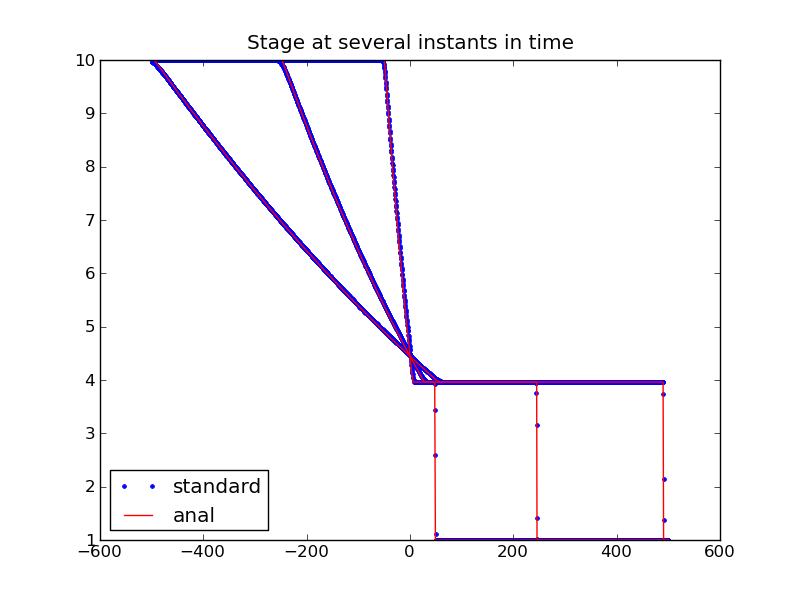
\includegraphics[width=0.9\textwidth]{stage_plot.png}
\end{center}
\caption{Stage results}
\end{figure}


\begin{figure}[h]
\begin{center}
\includegraphics[width=0.9\textwidth]{rmom_plot.png}
\end{center}
\caption{Radial momentum results}
\end{figure}


\begin{figure}[h]
\begin{center}
\includegraphics[width=0.9\textwidth]{rvel_plot.png}
\end{center}
\caption{Radial velocity results}
\end{figure}


\endinput
